\documentclass[12pt, titlepage]{article}

\usepackage{fullpage}
\usepackage[round]{natbib}
\usepackage{multirow}
\usepackage{booktabs}
\usepackage{tabularx}
\usepackage{graphicx}
\usepackage{float}
\usepackage{hyperref}
\hypersetup{
    colorlinks,
    citecolor=blue,
    filecolor=black,
    linkcolor=red,
    urlcolor=blue
}

\newcounter{acnum}
\newcommand{\actheacnum}{AC\theacnum}
\newcommand{\acref}[1]{AC\ref{#1}}

\newcounter{ucnum}
\newcommand{\uctheucnum}{UC\theucnum}
\newcommand{\uref}[1]{UC\ref{#1}}

\newcounter{mnum}
\newcommand{\mthemnum}{M\themnum}
\newcommand{\mref}[1]{M\ref{#1}}

\begin{document}

\title{\textbf{yoGERT GIS Toolbox}\\ Capstone 4G06\\ System Design Document}
\author{Team 19,
		\\ Smita Singh, Abeer Alyasiri, Niyatha Rangarajan,\\ Moksha Srinivasan, Nicholas Lobo, Longwei Ye \\\\
}
\date{\today}

\maketitle

\pagenumbering{roman}

\section{Revision History}

\begin{tabularx}{\textwidth}{p{3cm}p{2cm}X}
\toprule {\bf Date} & {\bf Version} & {\bf Notes}\\
\midrule
January 10th, 2023 & REV0 & Updated Sections 2-11, Moksha, Smita, Niyatha\\
January 18th, 2023 & REV0 & Revised based on MIS, Moksha, Niyatha \\
\bottomrule
\end{tabularx}

\newpage

\section{Reference Material}

\subsection{Abbreviations and Acronyms}

\renewcommand{\arraystretch}{1.2}
\begin{tabular}{l l} 
  \toprule		
  \textbf{symbol} & \textbf{description}\\
  \midrule 
   CLI & Command Line Interface\\
   ALs & Activity Locations are possible stop locations during an episode \\
   CSV & Comma Separated Values is a file type with data separated by commas. \\
   GIS & Geographical Information Systems\\
   GERT & GIS-based episode reconstruction toolkit \\
   Mode Detection (MD) & Detection of type of transportation being used \\
  \bottomrule
\end{tabular}\\

\newpage

\tableofcontents

\newpage

\listoftables

\listoffigures

\newpage

\pagenumbering{arabic}

\section{Introduction}
The following document is a high level system design document for the yoGERT software toolbox. The yoGERT toolbox is a reimplementation of the existing GERT toolbox that aims to aid geographers and the general public in processing and deriving insights from GPS data. For more information regarding this project please refer to the following: \\

\noindent\href{https://github.com/NicLobo/Capstone-yoGERT/blob/main/docs/SRS/SRS.pdf}{Link to Software Requirements Specification}\\
\noindent\href{https://github.com/NicLobo/Capstone-yoGERT/blob/main/docs/HazardAnalysis/HazardAnalysis.pdf}{Link to Hazard Analysis}\\
\noindent\href{https://github.com/NicLobo/Capstone-yoGERT/blob/main/docs/VnVPlan/VnVPlan.pdf}{Link to V\&V}\\


%\wss{Include references to your other documentation}

\section{Purpose}

The primary purpose of the system design document is to provide a high level overview of the toolbox's user interface and testing design decisions. Furthermore, it will include a thorough timeline for implementation. For more detailed, lower level design decisions, please refer to the documents below: \\

\noindent\href{https://github.com/NicLobo/Capstone-yoGERT/blob/main/docs/Design/SoftArchitecture/MG.pdf}{Link to Module Guide}\\
\noindent\href{https://github.com/NicLobo/Capstone-yoGERT/blob/main/docs/Design/SoftDetailedDes/MIS.pdf}{Link to Module Interface Specification}\\

%\wss{Purpose of your design documentation}
%\wss{Point to your other design documents}
\section{Scope}
\begin{figure}[!h]
    \centering
    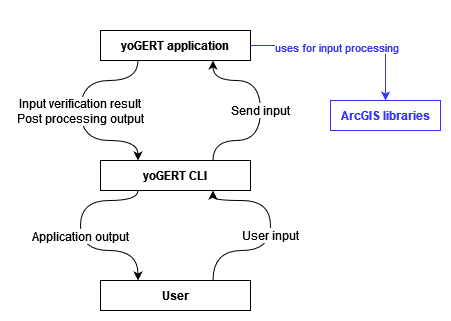
\includegraphics[width=0.6\linewidth]{REV0/SystDesign/sysdestcontextdiagram.png}
    \caption{System Context Diagram}
    \label{fig:System_Context_Diagram}
\end{figure}


\newpage
\section{Project Overview}

\subsection{Normal Behaviour}
Users will clone the yoGERT repo on github. Through the command line program of their choice (terminal, powershell, etc.), users will traverse to the yoGERT directory. From there, they will run the setup script within the home directory to update their environment and ensure correct version installation for all dependent libraries. Users may then use command line flags to upload their CSV GPS data for verification, the user will be presented with the following options:

\begin{itemize}
    \item[1.] Normalizing and Validating their GPS Traces
    \item[2.] Generate Travel Episode From GPS Traces
    \item[3.] Identify Activity Locations From Stop Episodes
    \item[4.] Generating Alternative Routes From Drive/Walk Episodes
\end{itemize}

\noindent Users will be directed to use a command based on the chosen task, users can choose the input directory and the name, format, and directory of the file(s) outputted from the chosen operation. For example, if the user would like to generate a travel episode, they can use the following command.



The user can then view the output in an external application, for example, Microsoft Excel for CSVs. 

\subsection{Undesired Event Handling}

%\wss{How you will approach undesired events}

\noindent A full analysis of the undesired event handling in the system can be found in the \href{../../HazardAnalysis/HazardAnalysis.pdf}{Hazard Analysis} document.\\

\noindent The main methods to handle undesired events are:
\begin{itemize}
    \item Robust documentation to help the user avoid any unauthorized or undefined actions
    \item A startup script to standardize the user's environment before running the toolbox
    \item Warnings provided to the user in the case of external environment factors (eg. too little memory for storage)
    \item Saving system state to avoid losing user data
\end{itemize}

\noindent If unexpected behaviour occurs, users will see error messages with recommended courses of action on their CLI. 

\newpage
\subsection{Component Diagram}
\begin{figure}[!h]
    \centering
    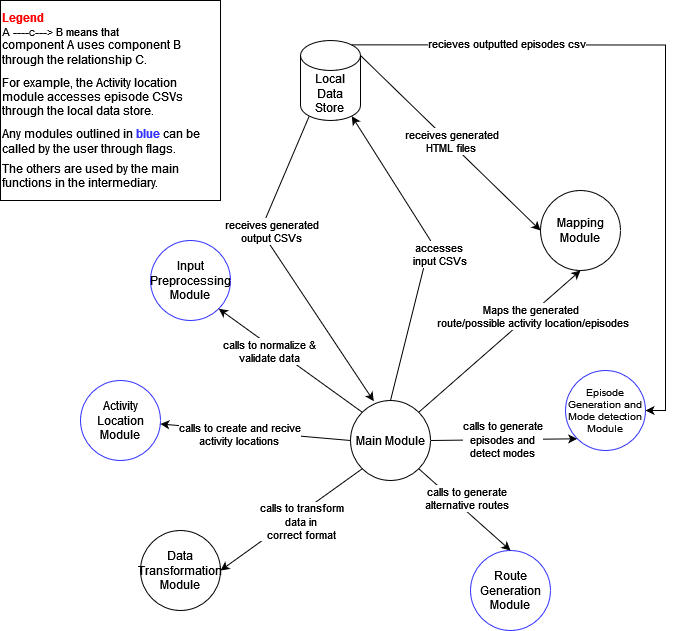
\includegraphics[width=0.88\linewidth]{REV0/SystDesign/systemcomponentdiagram.png}
    \caption{System Component Diagram}
    \label{fig:System_Component_Diagram}
\end{figure}

\newpage

\subsection{Connection Between Requirements and Design} \label{SecConnection}
R1: The system shall allow users to upload GPS data in a standard format - We are using a CSV format.\\

\noindent R2: The system shall process GPS data points. - we are creating episode segments that process GPS features through latitude and longitude\\

\noindent R4: The system shall produce output in a standard transferable format.- We are using a CSV format between processing per file.\\

\noindent R5: The system shall use longitude, latitude, and time variables from GPS data points. - we are using a CSV with those exact columns. \\

\noindent R6: The system shall extract episode attributes including speed, duration, direction, distance, change in direction, acceleration, and status points from GPS data points. - we have an episode generation function to achieve exactly this.\\

\noindent R8: The system shall classify extracted episode into different types including stop, car, walk, bus, and other travel episodes. - specified an enum type for detecting modes based on the velocity recorded.\\

\noindent R9: The system shall decompose episode into output segments of type stop and trip. - same as above.\\

\noindent R10: The system shall identify trip trajectory using extracted segments. - we have used the OSMNx library with Dijkstra's algorithm to match the points of interest with the shortest path taking into account the mode of travel.\\

\noindent R11: The system shall identify activity locations based on the episode attributes of the route to the stop point. - same as above\\

\noindent R16: The system shall store activity location identifications - mode generation handles this.\\

\noindent R18: The system shall allows requests for activity location description by filtering. - This description is possible using the OSMNx library.\\

\noindent R19: The system shall allow users to request trip segments’ description for a given GPS data set. - same as above\\

\noindent R20: The system shall allow users to request episode descriptions of GPS inputs - same as above \\

\noindent NFR2: The system shall display episodes through informative descriptions - same reasons for the OSMnx library.\\

\noindent NFR4: The system must be intuitive in terms of its design. - robust documentation in the set up script. As a user you only provide a CSV file and documentation explains how the CSV file will be processed.\\

\noindent NFR8: The system’s functionality must allow the user to track their progress. - The CSV files generated help track the progress per step. \\

\noindent NFR9: The system must render the require information within 6000 seconds upon request. - the OSMNx library is slow to load but caching the response allows to achieve this constraint.\\

\noindent NFR10: The system must not make the user’s location public. - It is a CLI that only uses local data. \\

\noindent NFR11: The system must render the route accurately matching the GPS data points provided. - we find the nearest node which validates the GPS trace on the shortest path.\\

\noindent NFR12: The system must be able to process 47.3 million points of GPS data. - this is possible through caching.\\

\noindent NFR15: The system shall be able to run on personal laptops and desktops that uses Linux, Windows, and MacOS operating system with Python preinstalled. - achieved since it is dependent on only python libraries.\\

\noindent NFR16: The system must be functional on Linux, Windows, and MacOS operating systems. - same as above.\\


*The numbering will be updated as the SRS is continues to be updated

% \wss{The intention of this section is to document decisions that are made
%   ``between'' the requirements and the design.  To satisfy some requirements,
%   design decisions need to be made.  Rather than make these decisions implicit,
%   they are explicitly recorded here.  For instance, if a program has security
%   requirements, a specific design decision may be made to satisfy those
%   requirements with a password.}
\newpage 
\section{System Variables}
\noindent N/A
%\wss{Include this section for Mechatronics projects}

\subsection{Monitored Variables}

\subsection{Controlled Variables}

\subsection{Constants Variables}

\section{User Interfaces}

\noindent The user will interface with the GERT toolbox through the use of their command line tool of choice (terminal, powershell, etc). This decision was partially driven by one of the main goals of the project, being able to process large inputs in a short amount of time. A CLI uses fewer system resources and thus allows for faster data processing. The other reason we chose a CLI is due to project time constraints, although a GUI would allow a wider range of users to interact with the system, the team simply does not have the time to implement a robust GUI. Lastly, conversing with the project supervisor, Dr. Paez, uncovered that many of the primary users (academics in the geography field) already have familiarity with the command line.\\

\noindent To ensure a seamless user experience, the team will document all possible user inputs with examples to follow along with. 

\section{Design of Hardware}
\noindent N/A

\section{Design of Electrical Components}
\noindent N/A

\section{Design of Communication Protocols}
\noindent The nature of our project did not facilitate the creation or design of a communication protocol as it is mainly a data transformation project. However, we did make some choices with regard to communication to minimize the likelihood of unexpected behaviour. We chose to use a wrapper for the OSM API called "overpy" rather than the API itself because we only require GETting information and never \textit{update} the open source database. This avoids accidental updates of the OSM database (although there is a thorough review process), especially when users try to manipulate the code.  \\

\noindent On the whole, our system follows a "pipe and filter" architecture style. This means that modules receive input from a data source, transform the data, and output the transformation. Although modules do interact, we ensured that large amounts of information are not being relayed through the modules. Instead, we store intermediate data sources for the user to peruse. \\

\section{Timeline}

\begin{table}[H] 
	\begin{tabularx}{\textwidth}{|X|X|X|}
		\hline
		\textbf{Module} & \textbf{Main Developer(s)} & \textbf{Due Date}\\
		\hline
		Input Pre-processing & Moksha Srinivasan & 
		January 24th, 2023  \\
		\hline
		Episode Generation & Nicholas Lobo & 
		January 24th, 2023 \\
		\hline
		Data Transformation & Moksha Srinivasan &
		January 25th, 2023 \\
		\hline
		Mapping Module & Niyatha Rangarajan &
		January 28th, 2023 \\
		\hline
		Alternative Route  & Abeer Al-Yasiri &
		January 29th, 2023 \\
		\hline
		Network Graph  & Abeer Al-Yasiri &
		January 29th, 2023 \\
		\hline
		Route Choice Generation & Abeer Al-Yasiri &
		January 29th, 2023 \\
		\hline
		Activity Location Detection & Smita Singh &
		January 30th, 2023 \\
		\hline 
		Travel Mode Detection & Nicholas Lobo & 
		January 30th, 2023 \\
		\hline 
		User Documentation & Longwei Ye &
		January 30th, 2023 \\
		\hline
		Setup Script & Moksha Srinivasan &
		January 31st, 2023 \\
		\hline 
		Main Module & Moksha Srinivasan &
		January 31st, 2023 \\
		\hline
	    Final Peer Code Reviews* & All &
		January 31st, 2023 \\
		\hline
		Integration Testing & Niyatha Rangarajan &
		February 1st, 2023 \\
		\hline
		Benchmark/Stress Testing & Longwei Ye & 
		February 2nd, 2023 \\
		\hline
	\end{tabularx}
	\caption{Module Timeline}
\end{table}

Before merging code, all team members will have written unit tests for their respective modules with mocked versions of the input ensuring correct module functionality. All components should be completed and tested by 1 week before the Final Demo on February 9th and changes made afterward will be for cleanup.\\

\noindent *Note: Although code reviews have been taking place throughout the implementation process, the team plans to come together and review code once again before the final demonstration. This ensure that code and documentation is all up to date and in line with changing requirements. 

\newpage{}

\appendix

\section{Interface}
\noindent No additional information 

\section{Mechanical Hardware}
\noindent N/A
\section{Electrical Components}
\noindent N/A
\section{Communication Protocols}
No additional information
\section{Reflection}

\noindent One limitation of yoGERT is the use of the OSM database to retrieve data regarding transportation networks, activity locations, and general up-to-date GPS data. Since the dataset is crowd-sourced, it is not updated as often as say, Google Maps and the toolbox with subsequently have inaccuracies. With unlimited resources, the yoGERT team would aggregate data from alternative sources such as the most recently updated local transportation maps to increase accuracy. \\

\noindent Furthermore, another limitation of the solution provided is the CLI interface. With more time and resources the team would be keen to create a front-end interface that is accessible to a wide variety of users. This is because a CLI tool can have a very high barrier to entry for non-technically oriented stakeholders. Furthermore, a GUI tool could more easily help students and those keen to learn about geoprocessing visualize the output.\\

\noindent Finally, one big limitation in our design of yoGERT is the inability to append to existing inputs and outputs. Since the system is batch sequential, in the current implementation it is not able to quickly update inputs and add new episodes. This functionality is achievable and very useful, but would require an overhaul of the current design to succeed. \\


\noindent Another design that the team explored was embedding the application into a Jupyter notebook. This aided in the mission of yoGERT being a learning tool, with full code transparency and markdown comments throughout. This allowed the user to understand exactly what is occuring as they run the code and gain an intuitive understanding of how to process and manipulate GPS data. However, the main drawback of this approach is that Jupyter notebook can be slow to start up and take a long time to execute code. One of the main goals of the toolbox is the ability to quickly process large amounts of data which is difficult using Jupyter notebook. The developers chose to stick with a CLI interface as it is significantly faster and those who are interested can still look through the documentation and manipulate the code accordingly. \\

\noindent Lastly, the team also explored using R to implement the toolbox. This was an idea suggested by the team's supervisor due to the language being designed for large scale data manipulation. The benefits of R would have been the ability to complete deep statistical analysis which is very useful for route choice analysis and mode detection. The disadvantages are that R has significantly fewer libraries for our use case (geography) and visualizations tend to be more robust in python. On the contrary, python is less efficient for deep statistical analysis but has significantly more libraries for our use case, and it is easier to provide interactive data visualizations. \\

\end{document}
